\chapter{Background in Reinforcement Learning}\label{ch:rl}

The field of reinformcement learning is large and growing. In this chapter we provide the background in reinforcement learning and modular reinformcenet learning necessary to understand our work and place it in context.

\section{Reinforcement Learning}

One can think of reinforcement learning (RL) \cite{sutton1998reinforcement,kaelbling1996reinforcement} as a machine learning approach to planning, that is, as a way of finding a sequence of actions that achieves a goal. In RL, problems of decision-making by agents interacting with uncertain environments are usually modeled as Markov decision processes (MDPs). In the MDP framework, at each time step the agent senses the state of the environment and executes an action from the set of actions available to it in that state. The agent's action (and perhaps other uncontrolled external events) cause a stochastic change in the state of the environment. The agent receives a (possibly zero) scalar reward from the environment. The agent's goal is to find a {\it policy}; that is, to choose actions so as to maximize the expected sum of rewards over some time horizon. An optimal policy is a mapping from states to actions that maximizes the long-term expected reward.  In short, a policy defines which action an agent should take in a given state to maximize its chances of reaching a goal.

\subsection{Markov Decision Processes}

The basic Markov decision process is a 3-tuple,

\begin{equation}
<S, A, T(s, a, s')>
\end{equation}

where

\begin{itemize}
\item $S$ is a set of states,
\item $A$ is a set of actions, and
\item $T(s, a, s')$ is a transition function which gives the probably that executing action $a$ in state $s$ will result in $s'$.
\end{itemize}

Most definitions of MDPS include a reward function, $R(s, a, s')$ which specifies the reward that the world provides to an agent for taking action $a$ in state $s$ and arriving in state $s'$ or, equivalently, a reward for arriving in state $s$, $R(s)$. Some definitions of MDPs include an initialization function, $I(s)$, which specifies the probablity the the agent will start in some state $s \in S$, others specify a particular state from $S$ as the start state.

We prefer to think of the basic 3-tuple MDP as representing the states and state transition dynamics of a world, and an agent solving a Markov Decision {\it Problem} which adds the reward function, initialization function, and discount factor. This distinction between Markov Decision {\it Processes} and Markov Decision {\it Problems} leads to a more natural expression of worlds and agents for programmers who are not familiar with the underlying theory of reinforcement learning. For example, most people would not include a single universal reward function as part of the ``world'' because different agents may value states differently. Similarly, different agents may have a shorter or longer term view of decision optimality and thus different discount factors. Separating the world dynamics from the agent's use of the world dynamics doesn't change the reinformcement learning algorithms, but as we will see in Chapter \ref{ch:afabl}, separating worlds from agents is useful in practical programming.

The solution to a Markov Decision Problem is a policy, denoted $\pi$, which is a mapping from states to actions. The policy says, for any state, what is the best action to take in order to maximaze the agent's long term reward.

\subsection{Long Term Reward}

Acting optimally in the world means maximizing your long term reward. In the MDP setting there are many ways to compute long term reward depending on whether you consider rewards gained during a finite or infinite time horizon, can depend on there being a terminal state the agent is guaranteed to reach, or whether the agent's task is episodic or continuing. The most commonly used formulation of long term reward is geometrically discounted rewards over an infinite time horizon, which works for episodic tasks, continuing tasks, and results in stationary policies, that is, policies that depend only on the current state no matter the time step in which the state is visited.

\begin{equation}
R_t = \sum_{k=0}^{\infty} \gamma^k r_{t+k+1}
\end{equation}

We use this conception of long term reward to calculate the values of states.

\subsection{Value Functions}

A value function assigns a number to each state indicating how good is it for an agent to be in that state. If you know the values of all the possible next states of your current state, then the action you should take is the action most likey to get you into the next state having the highest value.

The value of a state (or state, action pair) under a particular policy $\pi$ is the expected long term reward an agent would get starting from state $s$ if it followed $\pi$. The value is computed from the rewards and state transition dynamics of a world as follows:

\begin{equation}
V^\pi(s) = E \left [ \sum_{t=0}^{\infty} \gamma^t R(s_t) \right ]
\end{equation}

State value functions form the basis of dynamic programming approaches to solving MPDs. The reinforcement learning algorithms we discuss in Section \ref{sec:rl} use action value functions, which assign values directly to the actions available in a given state.

\subsection{Optimal Policies}

Since some states have higher values than others, and some actions have higher probabilities of causing transitions to higher-valued successor states, there is an optimal action in each state, namely, the action most likely to cause a transition to the highest-valued successor state. The optimal actions in each state is the optimal policy:

\begin{equation}
\pi^*(s) = \argmax_{a \in A} \sum_{s'} T(s, a, s') V(s')
\end{equation}

There may be many optimal policies for a given MDP, but without loss of generality we usually simply say ``the optimal policy.''

\subsection{Solving MDPs with Dynamic Programming}

If you have the MDP -- you know the transition function and reward function -- you can solve for the value of each state using value iteration, from which the optimal policy is derived, or find the policy directly using policy iteration. Although a practical reinforcement learning agent usually doesn't have the full MDP model, the theory of dynamic programming is useful in understanding reinforcement learning algorithms.

\subsubsection{Value Iteration}

Previously we defined the value of a state under a particular policy. If we assume the optimal policy, we can define the maximum value of a state in terms of optimal actions:

\begin{equation}
V(s) = R(s) + \max_{a \in A} \sum_{s'} T(s, a, s') V(s')
\end{equation}

This equation is called the Bellman optimality equation. There is one Bellman equation for each state -- $n$ equations in $n$ unknowns (the values) for a state space of size $n$. However, since the $max$ operator is nonlinear we cannot solve the system of simultaneous Bellman equations using linear algebra. One solution is to use an iterative dynamic programming approach: value iteration. The value iteration algorithm initializes each state values to random values, then iteratively update these values by turning the Bellman equation into an update rule (the Bellman update):

\begin{equation}
V_{i+1}(s) \leftarrow R(s) + \max_{a \in A} \sum_{s'} T(s, a, s') V(s')
\end{equation}

These updates are applied at the same time for all states, i.e., the values in iteration $i+1$ are calculated from the values in iteration $i$. The value iteration algorithm is listed in Algorithm \ref{alg:value-iteration}


\begin{algorithm}
  \caption{Value Iteration}\label{alg:value-iteration}
  \begin{algorithmic}
    \State $V \gets$ random initial values
    \Repeat
      \State $V' \gets V$
      \For{each $s \in S$}
        \State $V'(s) \gets R(s) + \max_{a \in A} \sum_{s'} T(s, a, s') V(s')$
      \EndFor
      \State $V \gets V'$
    \Until $V$ changes by a sufficiently small amount
  \end{algorithmic}
\end{algorithm}

If we apply the Bellman update infinitely often, then value iteration reaches an equilibrium at which point the values of the states are solutions to the Bellman equations, that is, they are optimal. A policy derived from these values is an optimal policy.

In practice we may iterate until the updated values change by a sufficiently small amount. If all we care about is finding the optimal policy, then it doesn't matter that we find the optimal values, only that the values we find lead to the same optimal policy.

\subsubsection{Policy Iteration}

In policy iteration we start with a random initial values and policy and alternate between two steps for each iteration $i$:

\begin{itemize}
\item {\bf Policy evaluation.} Use policy $\pi_i$ to calculate the values of of each state using the duscounted current values of their successor states. Since we are calculating the values under a particular policy, we drop the $max$ operator:

  \begin{equation}
  V_{i+1}(s) = R(s) + \gamma \sum_{s'} T(s, a, s') V(s')
  \end{equation}

\item {\bf Policy improvement.} Calculate policy $p_{i+1}$ using the values calculated in the previous step.
\end{itemize}

When policy improvement does not change the policy, an optimal policy has been found and policy iteration terminates.

Note that since the update equation used in policy evaluation is linear, we can use linear algebra to solve the set of simultaneous linear equations in $O(n^3)$. This method works fine for smaller state spaces but may be too expensive for large state spaces. A solution to this problem is known as modified policy iteration, which combines policy iteration with value iteration by using a bounded number of Bellman updates to perform the policy evaluation step.

\subsection{Learning Policies via Reinforcement Learning}\label{sec:rl}

If the agent doesn't have the model, then the agent must learn a behavior policy by interacting with the world by taking actions, observing the effects of these actions (state transitions and reward signals), and using these observations to update some model of the world that can be used to guide future behavior. Unlike the MDP solvers discussed previously which calculate values for every state in every iteration, reinforcement learning agents choose which states to visit and often do not visit every state, leading to a central issue in refinforcement learning: exploration vs. exploitation.

\subsubsection{Exploration versus Exploitation}

Exploration means visiting some state of the world you haven't yet visited. Eating at a restaurant or ordering a dish you haven't tried to see if you like it is an example of exploration. Exploitation means using knowledge already learned. Eating a dish you know you like at a restaurant you know you like is an example of exploitation. The exploration versus exploration question is one of risk versus reward: exploration risks wasting effort on a possibly bad outcome, explotation trades that risk for a known reward but risks missing a discovery of something better.

In the case of reinforcement learning agents exploration means taking an action in a state that may take the agent to a state not yet visited. Exploitation means using the agent's current value estimates to choose an action. We call exploitation {\it greedy} action selection becuase it chooses an action that is likely to result in higher reward. There is a saying in machine learning: the less you know the less you should trust your knowledge, the more you know the more you should trust your knowledge. A reinforcement learning agent should favor exploration early in its learning process and explotation after its model of the world stabilizes.

Implementing an exploration strategy in a reinforcement learning algorithm can be done using softmax action selection such as a Boltzmann distribution, which uses a decaying temprature parameter similar to annealing to gradually decrease the randomness of action selection, or by a simpler method known as $\epsilon$-greedy action selection.  $\epsilon$ is a real number in $(0, 1)$ that represents the probability of choosing an action randomly (exploring). $\epsilon$ is decayed over time so that action selection favors exploration early in the learning process and exploitation later. We use $\epsilon$-greedy action selection in our algorithm implementations.

\subsubsection{Q-Learning}

An alternative value function assigns values to state-action pairs instead of states. Such a function is called a {\it Q-function}, and the optimal Q-function is defined as:

\begin{equation}
Q*(s, a) = \gamma \sum_{s'} T(s, a, s') \max_{a'} Q(s', a')
\end{equation}

which means that the value of taking action $a$ in state $s$ is the reward received from state $s$ plus the discounted probabilistic sum of the Q-values of successor states assuming that optimal successor actions $a'$ are taken in the successor states $s'$.

An important consequence of learning a Q-function instead of a state-value function is that, although Q-values can be defined as above, a reinforcement learning agent can approximate the Q-function using temporal difference learning which does not require the model. A reinforcement learning agent only needs to know the Q-values because the purpose is only to learn a policy which is derived directly from the Q-function. This is the idea behind the Q-learning algorithm, which uses the following temporal difference update rule:

\begin{equation}\label{eqn:q-update}
Q(s, a) \leftarrow Q(s, a) + \alpha [R(s) + \gamma \max_{a'} Q(s', a') - Q(s, a)]
\end{equation}

$\alpha$ is a learning rate parameter. Temporal difference algorithms like Q-learning use the differences between Q-values in successive states to update Q-values in each iteration. Like value and policy iteration, Q-learning has been shown to converge to $Q*$ in the limit with infinite exploration. In practice developing a close approximation to $Q*$ isn't necessary as long as the same policy results.

\begin{algorithm}
  \caption{General Q-Learning}\label{alg:q-learning}
  \begin{algorithmic}
    \State $Q \gets$ random initial values
    \For{each episode}
      \State $s \gets$ world.initialState()
      \Repeat
        \State $a \gets \epsilon-$greedy action for $s$ from $\pi$ derived from $Q$
        \State Execute $a$, observe effects $r$ and $s'$
        \State $Q(s, a) \gets Q(s, a) + \alpha [R(s) + \gamma \max_{a'} Q(s', a') - Q(s, a)]$
        \State $s \gets s'$
      \Until $s$ is terminal
    \EndFor
  \end{algorithmic}
\end{algorithm}


\subsubsection{Sarsa}

Because it uses the best successor Q-value in its update rule, Q-learning is an off-policy learning algorithm, meaning that it does not use the policy being followed by the agent. A close relative of Q-learning is the SARSA algorithm, which is an on-policy algorithm that uses the following update rule:

\begin{equation}\label{eqn:sarsa-update}
Q(s, a) \leftarrow Q(s, a) + \alpha [R(s) + \gamma Q(s', a') - Q(s, a))]
\end{equation}

Sarsa gets its name from the elements of its update rule: $s$, $a$, $r$, $s'$, $a'$. The key difference is that the $Q(s', a')$ from the agent's policy is used in the update rule.

\begin{algorithm}
  \caption{General Q-Learning}\label{alg:sarsa}
  \begin{algorithmic}
    \State $Q \gets$ random initial values
    \For{each episode}
      \State $s \gets$ world.initialState()
      \State $a \gets \epsilon-$greedy action for $s$ from $\pi$ derived from $Q$
      \Repeat
        \State Execute $a$, observe effects $r$ and $s'$
        \State $a' \gets \epsilon-$greedy action for $s'$ from $\pi$ derived from $Q$
        \State $Q(s, a) \gets Q(s, a) + \alpha [R(s) + \gamma Q(s', a') - Q(s, a))]$
        \State $s \gets s'$
        \State $a \gets a'$
      \Until $s$ is terminal
    \EndFor
  \end{algorithmic}
\end{algorithm}

Q-learning has the advantage of being able to learn an optimal policy even if the control policy during learning is poor. The advantage of Sarsa over Q-learning is that if the agent does not have full control over action selection selection, Sarsa will learn a policy that is optimal in the presence of external control over action selection, such as other (sub)agents. For this reason, Sarsa is used in modular reinforcement learning.

\section{Decompositional Reinforcement Learning}

Decomposition is an imortant tool in designing software systems in general, and as we'll see in Section \ref{sec:curse-dimensinality} a necessity for larger state spaces likely to be envcountered in real-world problems. Hierarchical refinforcement learning (HRL), discussed first below, has had as a primary goal improved authoring based on temporal subgoals that allows intermediate tasks to be modeled as higher-level actions. HRL has also formed to basis of current approaches to RL-based programming systems. Modular reinforcement learning (MRL) decomposes the original problem concurrently, modeling an agent as a set of concurrently running reinforcement learning modules. MRL has been used primarily to model multiple-goal problems and to deal with large state spaces. This work is the first to use MRL as the basis of a practical programming system.

\subsection{Hierarchical Reinformcement Learning}

Current implementations of partial programming are based on hierarchical reinforcement learning (HRL), which exploits a temporal decomposition of the Q function.  In the case of HRL, the designer typically specifies a delegation hierarchy of components with points of adaptation where a policy is learned to perform the delegation.  The designer programs the policies of some of these components, which constitute a partial specification of the agent's behavior, and some of the components use reinforcement learning to adapt to the hierarchy by learning the control policies for their parts of the problem.  The adaptive components relieve the designer from writing the parts of the program that are hard to specify, or require difficult to write adaptivity, and the partial program constrains the learning problem faced by the adaptive components, which speeds convergence.  Components can be reused in other contexts, providing for modularity in temporal problem decompositions.

The current state of the art in HRL is based on the theory of {\bf Semi-Markov Decision Processes} (SMDPs). In an SMDP some actions are allowed to take more than one time step. These multi-step actions, sometimtes called macros, subroutines, options, or hierarchical machines represent a form of procedural abstraction that may allow a programmer to write reinforcement learning agents in a manner similar to writing other kinds of computer programs. The SMDP-based thread of reasearch in HRL also includes work in developing programming languages and systems that exploit HRL models, making this line of research particularly relevant to our work.

Precup's {\bf Options} \cite{precup1998a-theoretical,sutton1999between,precup2000a-temporal} framework develops a detailed theory of temporal abstraction abstraction based on SMDPs which include inter-option . Dietterich's {\bf MAXQ} \cite{dietterich1998maxq,dietterich2000hierarchical} and {\bf Hierarchical Abstract Machines} \cite{parr1998reinforcement} models decompose an MDP into a hierarchies of smaller MDPs. These smaller MDPs represent {\it subroutines} in the MAXQ framework or {\it HAMs} in the {\it Hierarchical Abstract Machines} framework. Andre's {\bf Programmable Hierarchical Abstract Machines} \cite{andre2000programmable,andre2002state} develops a programming language for HAMs called ALisp (Adaptive Lisp), and Marthi and colleagues  \cite{marthi2005concurrent} extend ALisp (Concurrent ALisp) for single reinforcement learning agents with multiple simultaneous actions, such as as robots with multiple effectors or a controller for multiple characters in a computer game.

\subsection{The Curse of Dimensionality in Reinforcement Learning}\label{sec:curse-dimensinality}

As with other kinds of machine learning, reinforcement learning must deal with the curse of dimensionality. In reinforcement learning the curse of dimensionality manifests itself primarily in the size of the state space, namely, the state space grows exponentially in the number of state features. As an example, consider the $5 \times 5$ grid of the bunny world in Figure \ref{fig:bunny-world}.

\begin{figure}[h]

\begin{center}
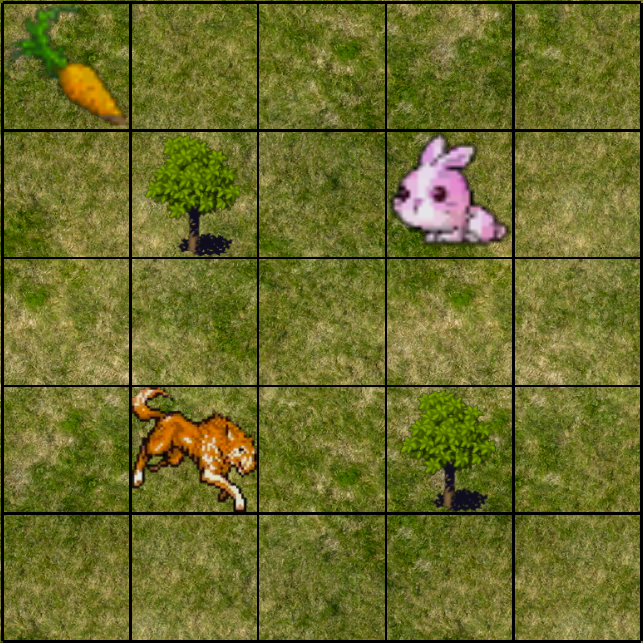
\includegraphics[height=2.4in]{bunny.png}
\end{center}
\caption{In the grid world above, the bunny must pursue two goals simultaneously: find food and avoid the wolf.  The bunny may move north, south, east, or west.  When it finds food it consumes the food and new food appears elsewhere in the grid world, when it meets the wolf it is eaten and ``dies.''}
\label{fig:bunny-picture}
\end{figure}

The bunny, food, and wolf can be in one of 25 possible states. If the task of the bunny were only to reach a particular state, then the number of states woudl be 25. But if you add the task of avoiding a wolf that pursues the bunny, then the state space gros to $25^2 = 625$. Add the food that reappears in a new location after it is found and ``eaten'' and the state space grows to $25^3 = 15625$. If you model this problem as two separate modules, one in which the bunny avoids the wolf and another in which the bunny finds food, then each module solves a problem with a state space of $25^2 = 625$ states (bunny plus wolf and bunny plus food).

\subsection{Modular Reinforcement Learning}\label{sec:mrl}

A second kind of decomposition in reinforcement learning, which is somewhat confusingly referred to as modular reinforcement learning (MRL) ~\cite{russell2003q-decomposition,sprague2003multiple-goal}, decomposes the original problem {\it concurrently} rather than temporally. Instead of composing sequential actions into action sequences, a MRL agent is decomposed into several modules each of which is concurrently learning a different subgoal of the original, complex, multiple-goal learning problem. The architecture of an MRL agent is reminiscent of Brooks's subsumption architecture, where an agent is decomposed into several modules that each receive sensor input and each independently suggest an action for the overall agent to take. As we will soon discuss, our approach uses Brooks's idea of a central arbitrator to choose the agent's actions from the suggestions of its modules.

There have been two major kinds of approaches to modular reinforcement learning: merging MDPs \cite{singh1998how-to-dynamically}, and merging Q functions \cite{sprague2003multiple-goal,russell2003q-decomposition}. Since we are interested in applying reinforcement learning in practical domains where we can't assume, or don't want to require, complete knowledge of the world's state transition dynamics, we focus on approaches to MRL that merge Q-functions.

In an MRL agent each module observes the action taken by the agent, the state transaition and a reward signal specific to the module. On each occasion that a decision for what action to take is needed, the agent combines the action preferences of the modules to compute the output of the joint policy.  The current state of the art in modular reinforcement learning uses the the Q-values of the modules directly to effect this action selection. The joint policy is derived from a joint Q-function in which the Q-values for each module are added.

\begin{equation}\label{eqn:joint-q}
  Q_{joint}(s, a) = \sum Q_i(s, a)
\end{equation}

Russel's and Zimdars' Q-decomposition \cite{russell2003q-decomposition} is equivalent to Sprague and Ballard's GM-Sarsa \cite{sprague2003multiple-goal}. In this work we will refer mostly to GM-Sarsa. Both of these investigations of Q-function (de)composition showed that Sarsa is a better choice for agent modules than Q-learning because Sarsa is on-policy. As we discussed earlier, Sarsa updates its Q-function based on the policy being followed by the agent where as Q-learning updates its Q-function assuming the optimal policy will be followed. Because modules do not have direct control over the policy being followed, on-policy learning algorithms like Sarsa perform better. For this reason, and so we can compare directly to GM-Sarsa, we also use Sarsa in our modules.

There is clearly a desire to model agents with multiple goals represented as reinforcement learning modules. We list only a few examples here. Sprague and Ballard have applied GM-Sarsa to problems in eye movement scheduling \cite{sprague2003eye,sprague2007modeling}. Konidaris and Barto applied an algorithm derived from GM-Sarsa to adaptive robot control \cite{konidaris2006adaptive}. Aissani and colleagues used GM-Sarsa to develop a system for dynamic scheduling of maintenance tasks in the petroleum industry \cite{aissani2009dynamic,chaari2014scheduling}. Rowe and colleagues used GM-Sarsa for interactive narrative planning \cite{rowe2013modular}. All of the work applying MRL has been done by single teams of researchers applying MRL to research problems. Thus, modules were authored together with comparable reward scales. To support reusability in a software engineering sense we need to support the separate authoring of modules. Separately authored modules may use reward scales that are internally consistent within modules but incomparable to the rewards used in other modules. In the next chapter we show that existing approaches to MRL degrade when modules use incomprable reward scales and present an algorithm that does not exhibit the same degredation.
